\chapter{Introdução}

Neste relatório iremos mostrar e explicar os resultados obtidos da análise de dois ficheiros distintos (www.fct.unl.pt.csv e bigFlows.csv) respondendo às perguntas especificadas do enunciado fornecido. Todos os tópicos foram implementados desde as obrigatórias (a1, a2, a3, a4 e a5) às opcionais (b1, e b2).

A implementação deste enunciado é escrito em código Python na sua versão 3 \cite{PYTHON3}, tendo sido também usada uma API externa e um ficheiro auxiliar, para a Geolocalização \cite{API} (IPGeolocation.py) e listagem das portas TCP e UDP \cite{PORTS} respectivamente. O uso da API requis uma autenticação, pelo que usamos as nossas contas Gmail da faculdade para obter as chaves necessárias (estando estas \textit{
harcoded} nos ficheiros necessários)

Inicialmente começamos por implementar um \textit{script} (intoDB.py) para inserir todos os dados do ficheiro .csv para uma base de dados relacional (SQLite \cite{SQLite}) de forma a mais tarde poder-mos fazer as perguntas utilizando SQL. Esta abordagem posteriormente não foi utilizada, porque achamos que talvez fosse mais confuso. Então decidimos manter o ficheiro intoDB.py para eventuais trabalhos de otimização futuros caso estes fossem necessários.

Nos tópicos opcionais (b1 e b2) optamos por criar os gráficos pretendidos utilizando a biblioteca \textit{matplotlib} \cite{MAT} de modo a converter a nossa informação em forma de mapa (key value) em gráficos 2D.

De seguida iremos, em cada capitulo, mostramos os nossos resultados para cada tópico do enunciado, falando da nossa abordagem ao problema e forma como esta foi implementada.

Inicialmente começamos por implementar uma estratégia de leitura dos ficheiros, onde abrimos o ficheiro pretendido iterando linha a linha a informação nele contida. O formato deste código foi repetido para os diferentes \textit{scripts} de modo a facilitar e dividir cada tópico pretendido.

\clearpage

Cada coluna, em termos de código, será representada da seguinte forma:
\begin{itemize}
    \item row[0] = time start
    \item row[1] = time end
    \item row[2] = duration (s)
    \item row[3] = source address
    \item row[4] = destination address
    \item row[5] = source port
    \item row[6] = destination port
    \item row[7] = protocol
    \item row[8] = flags
    \item row[9] = packets
    \item row[10] = bytes
\end{itemize}

Na figura 1.1 podemos ver esta parte do \textit{script} comum a todos os ficheiros implementados, não sendo esta mais falava nos próximos capítulos por motivos de repetição:

\begin{figure}[h]
    \label{high}
    \centering
    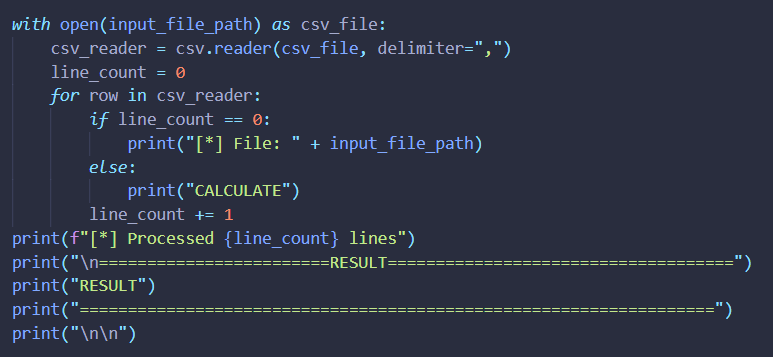
\includegraphics[width=1\textwidth]{Images/reader.png}
    \caption{\textit{Código inicial para cada tópico}}
\end{figure}

\textbf{Nota:} O código está num repositório GitHub privado, pelo que caso queira ter acesso ao mesmo deverá enviar um email aos autores a pedir autorização de acesso.

Link: \textbf{\url{https://github.com/rfa-lopes/APRC}}